\documentclass{beamer}
\definecolor{links}{HTML}{2A1B81}

\usepackage[utf8]{inputenc}
\usepackage[norsk]{babel}
\usepackage{hyperref}
\hypersetup{
  colorlinks=true,
  linkcolor=,
  urlcolor=links
}

\usetheme{Copenhagen}
\usecolortheme{seahorse}

\title{Bibliotekorientering}
\author{Thomas Rambø\inst{1}}
\institute[DMMH-biblioteket]{
  \inst{1}
  Biblioteket\\
  Dronning Mauds Minne Høgskole
}

\date[DMMH 2018]{DMMH, høsten 2018}
\logo{
\includegraphics[height=1.5cm]{media/logo.png}}

\begin{document}

\frame{\titlepage}
\begin{frame}
  \frametitle{Innhold}
  \tableofcontents
\end{frame}

\section{Velkommen til biblioteket}
\begin{frame}
  \frametitle{Velkommen til biblioteket}
  \centering
  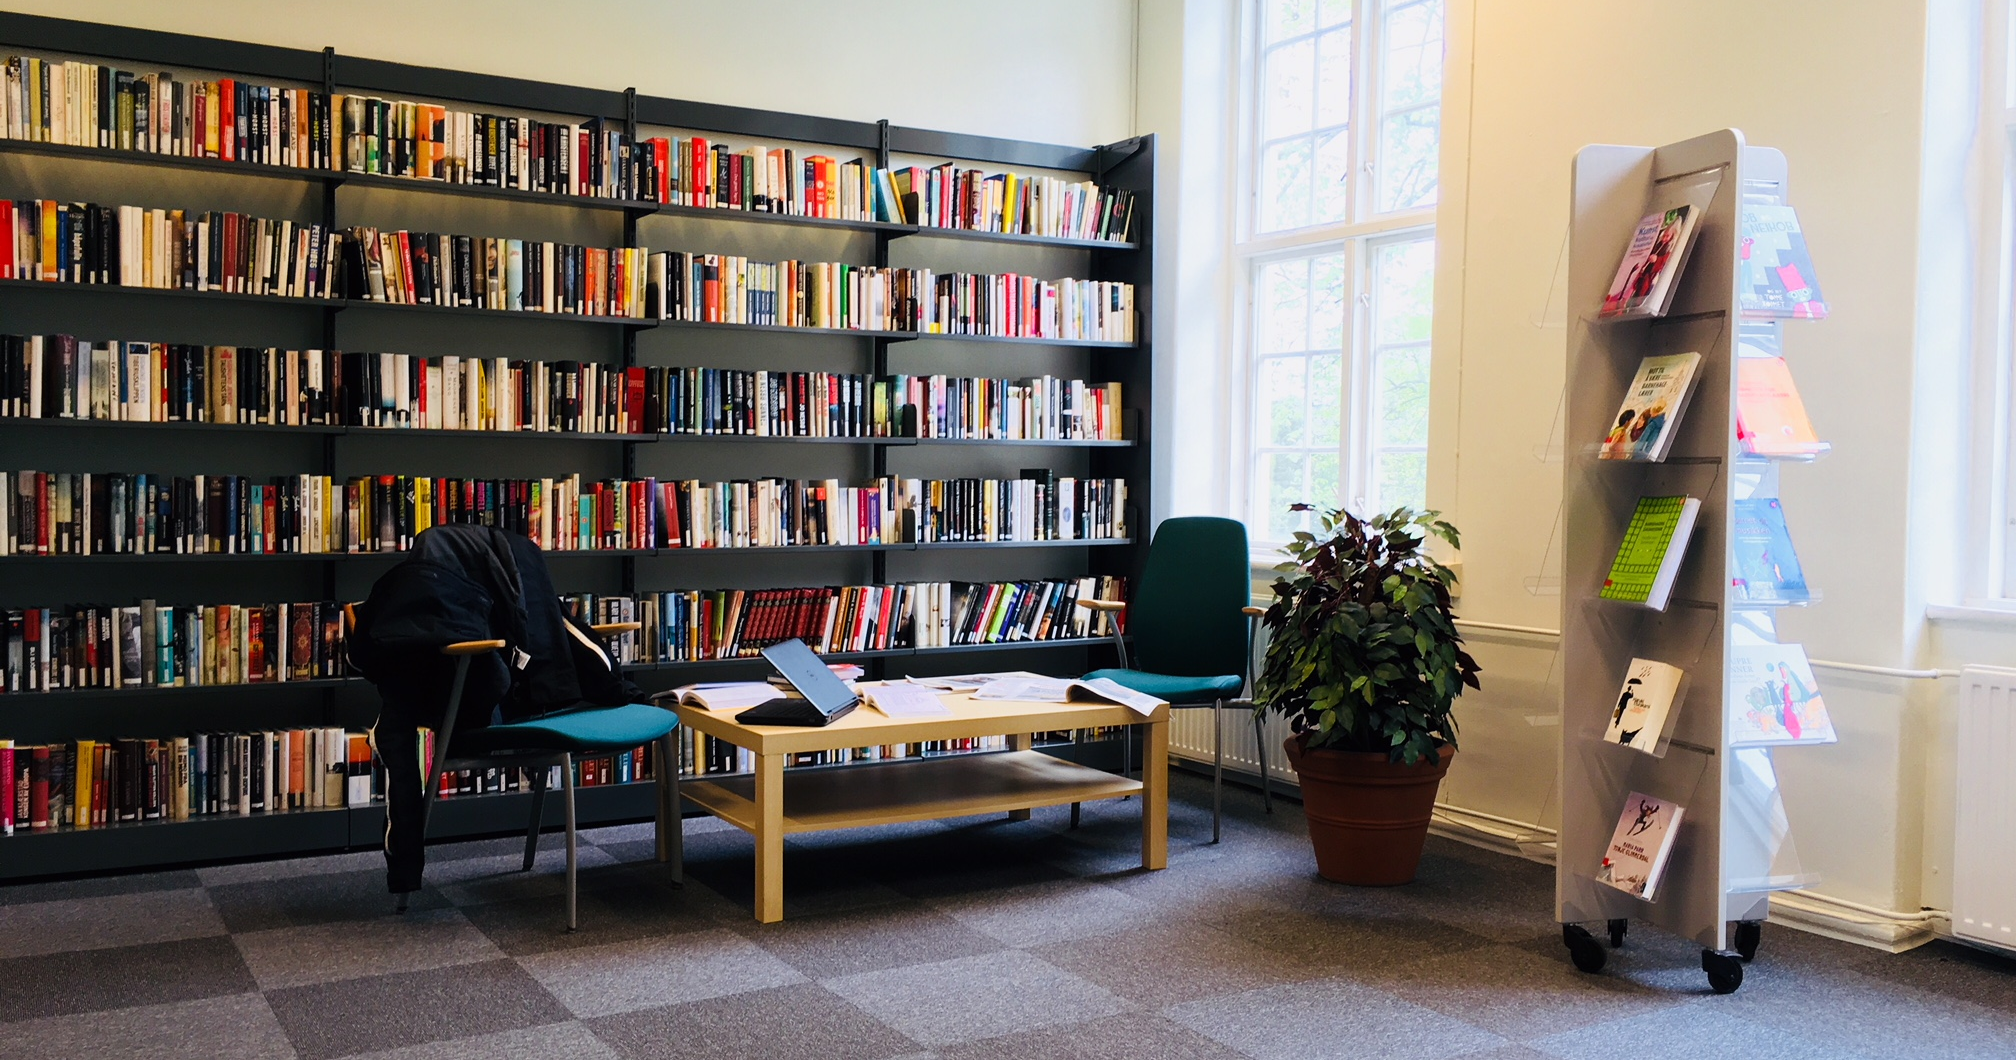
\includegraphics[width=0.90\textwidth]{media/nytt-bibliotek.png}
\end{frame}
\begin{frame}
  Biblioteket ligger i 2. etasje i hovedbygget, og holder åpent mandag til fredag. Mandager og onsdager er åpningstidene \alert{08:30 til 19:00}, og ellers er åpningstidene \alert{08:30 til 15:30}.
\end{frame}
\begin{frame}
  Personalet på biblioteket er på jobb for å bistå deg.

  \vfill
  \begin{tabular}{ l | l }
    Besøk oss: & Biblioteket ligger i 2. etasje i hovedbygget. \\
    På Facebook: & \url{https://m.me/dmmhbib} \\
    Telefon: & \texttt{73 80 52 42} \\
    E-post: & \url{mailto:bibliotek@dmmh.no}
  \end{tabular}
\end{frame}

\section{Hvilke tjenester kan biblioteket tilby?}
\subsection{Pensumlitteratur og annen støttelitteratur}
\begin{frame}
  \frametitle{Pensumlitteratur og annen støttelitteratur}
  Bibliotekets samling består blant annet av \alert{pensumlitteratur} og annen \alert{støttelitteratur}. Det er flere eksemplarer tilgjengelig, og som regel ett eksemplar som bare kan leses i bibliotekets lokaler.

  \vfill

  \begin{block}{Bemerkning}
    Bruk søketjenesten \href{http://bibsys-almaprimo.hosted.exlibrisgroup.com/primo_library/libweb/action/search.do?vid=DMMH}{Oria} til å finne fram litteraturen.
    \textit{Nesten} alt finnes i Oria.
  \end{block}
\end{frame}

\subsection{Vitenskapelig arkiv}
\begin{frame}
  \frametitle{Vitenskapelig arkiv}
  \begin{columns}
    \column{0.5\textwidth}
    I den digitale samlingen har vi et \href{https://brage.bibsys.no/xmlui/handle/11250/92951}{vitenskapelig arkiv} med forskningsresultater fra DMMH og fremragende studentoppgaver.

    \column{0.5\textwidth}
    \begin{figure}
      \caption{Forsiden av en bacheloroppgave i BIBSYS Brage.}
      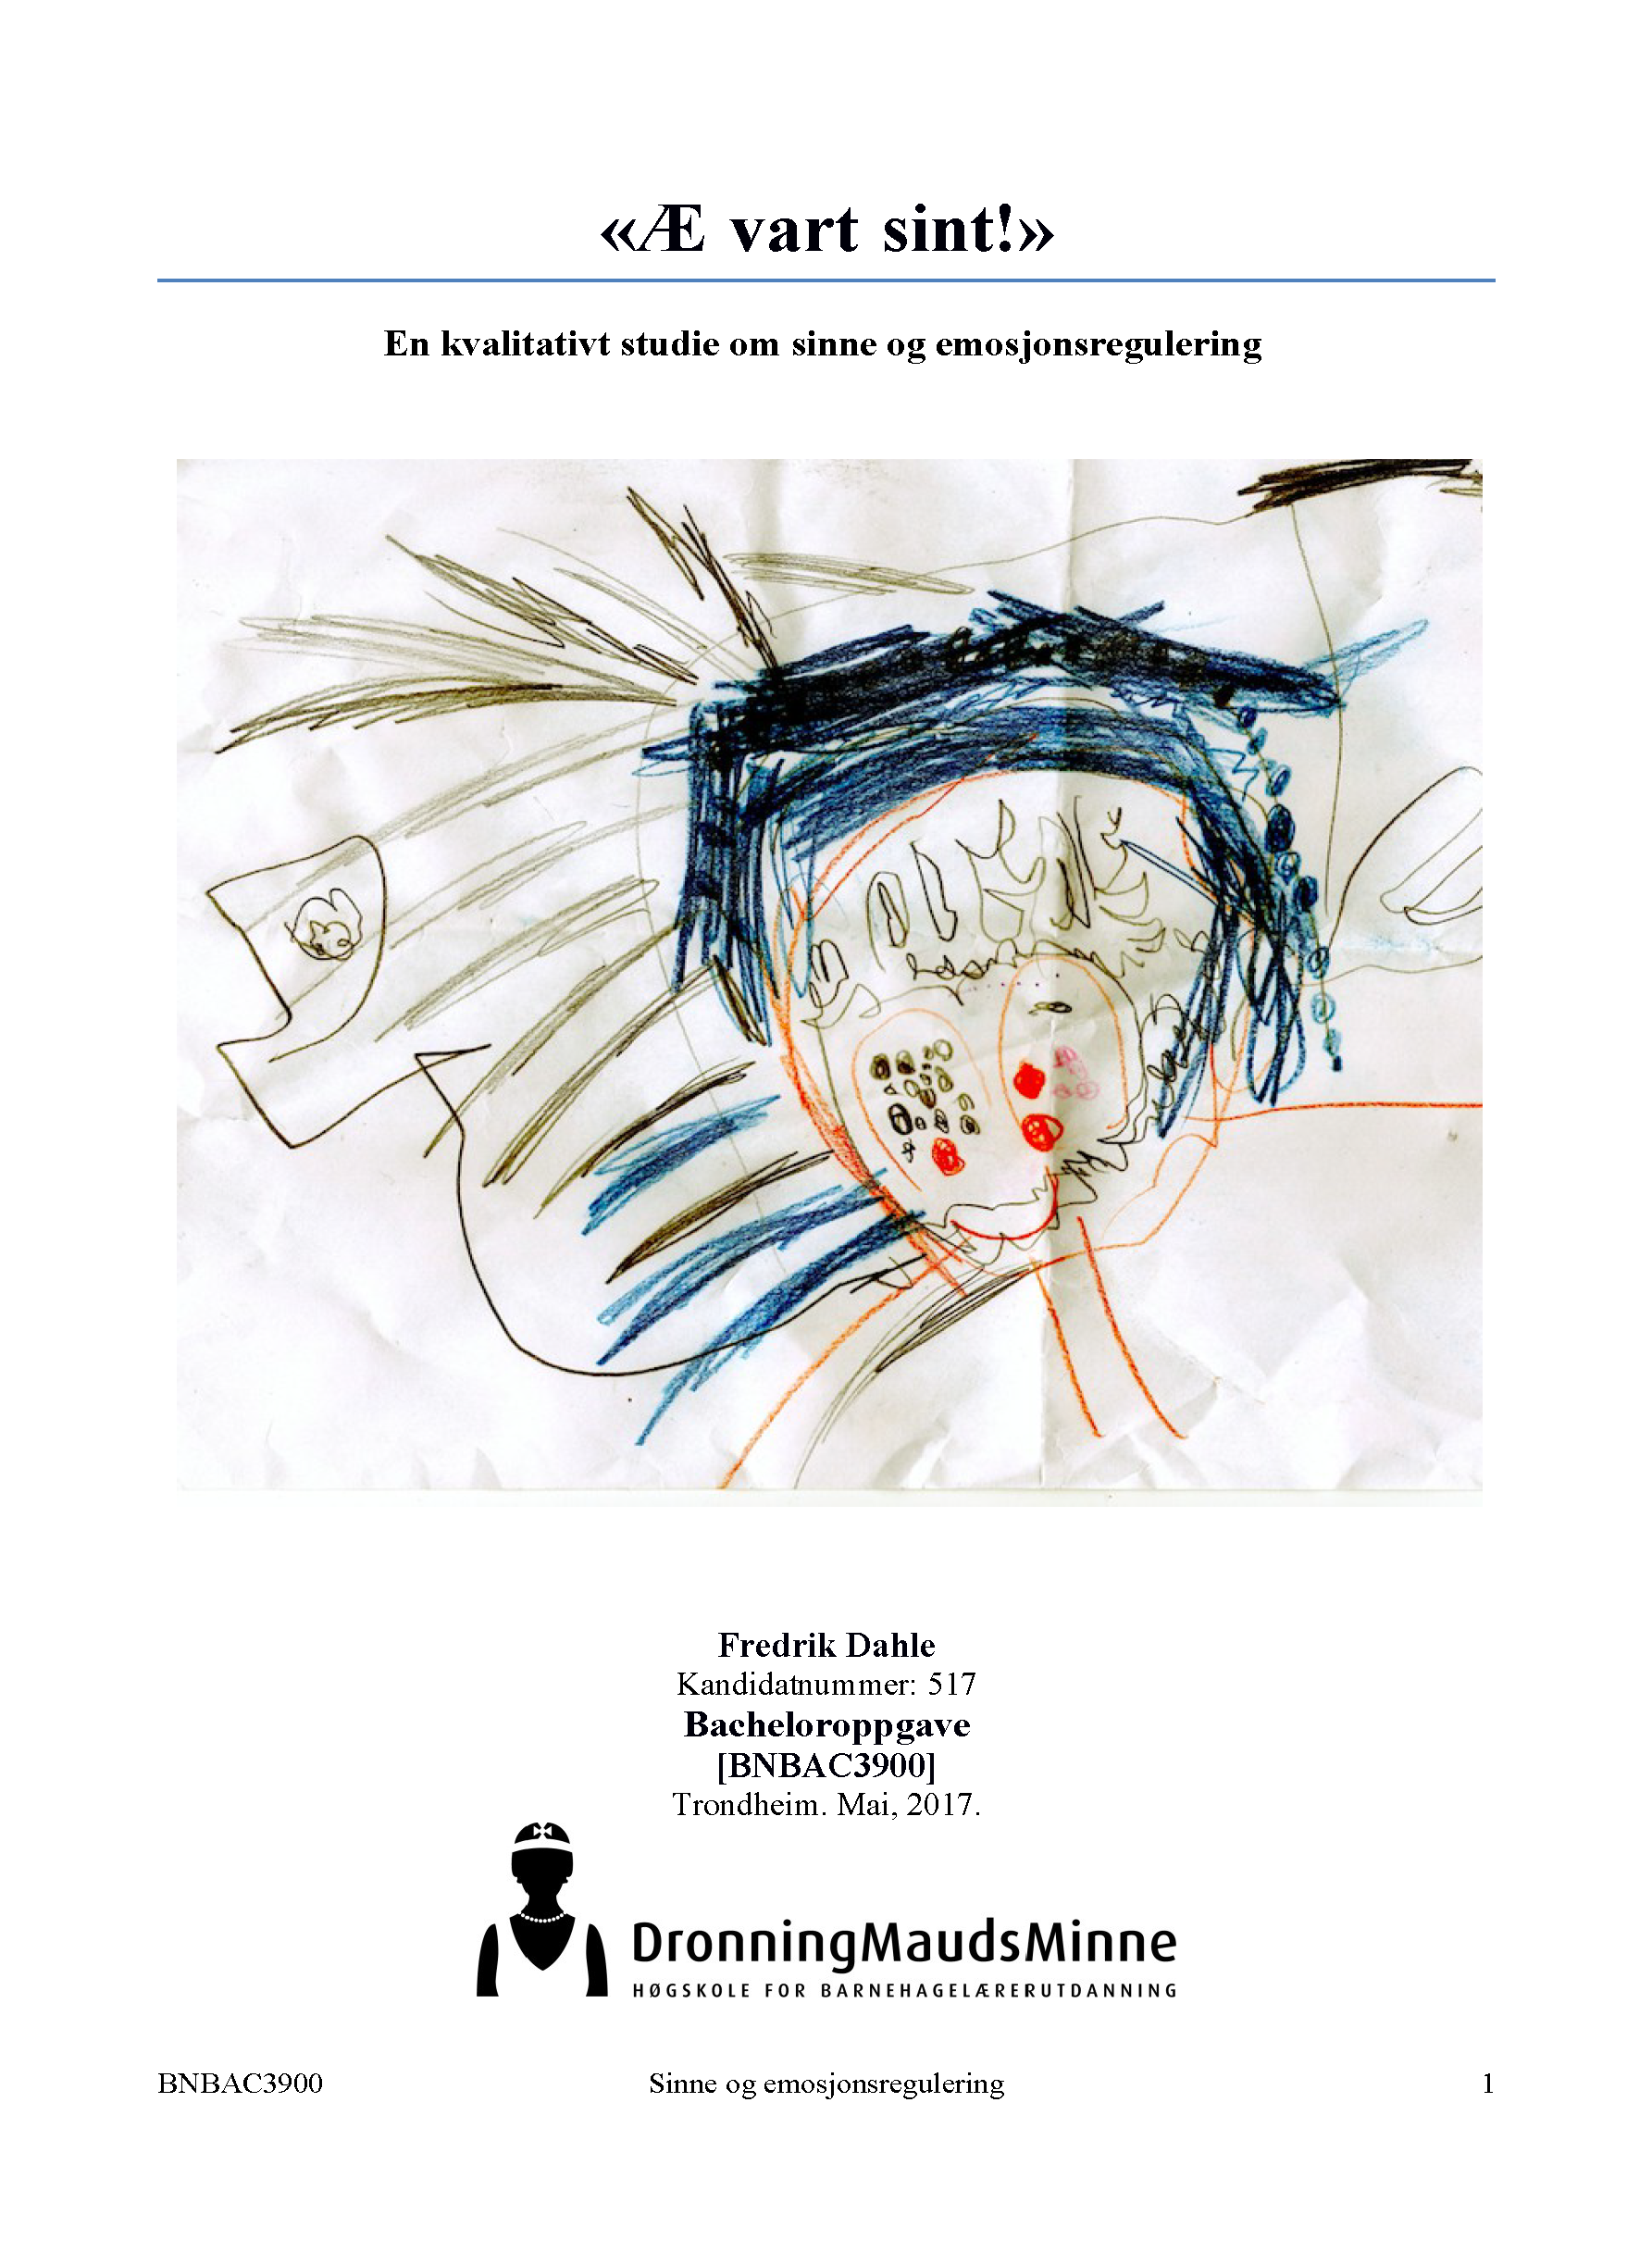
\includegraphics[width=0.5\textwidth]{media/front-dahle.png}
    \end{figure}
  \end{columns}
\end{frame}

\subsection{Bibliografisk veiledning}
\begin{frame}
  \frametitle{Bibliografisk veiledning}
  På Dronning Maud brukes en spesifikk \alert{referansestil} på sitering og bibliografier i studentoppgaver. Denne er basert på APA 6. utgave, og biblioteket kan besvare spørsmål om riktig referering og bibliografisk utforming.

  \vfill

  \begin{block}{Bemerkning}
    Nettjenesten \href{https://sokogskriv.no/}{Søk \& Skriv} har nyttig informasjon om det å skrive oppgaver og hvordan man setter opp en referanseliste.
  \end{block}
\end{frame}
\begin{frame}
  \frametitle{Referansehåndteringsverktøyet Zotero}
  \begin{columns}
    \column{0.5\textwidth}
    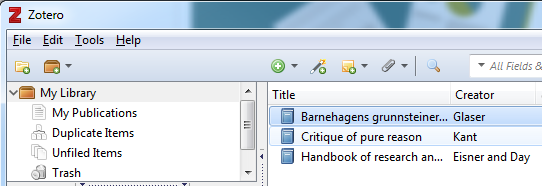
\includegraphics[width=1\textwidth]{media/zotero.png}
    
    \column{0.5\textwidth}
    Referansehåndteringsverktøy kan strukturere og ordne referanselister og siteringer i oppgaver. \href{https://dmmh.no/bibliotek/skriving-og-referering/zotero}{Zotero} er gratis og kan automatisk opprette referanser fra innførsler i bibliotekkatalogen, litteraturdatabaser og ordinære nettsider. Zotero støtter norsk APA 6. utgave.
  \end{columns}
\end{frame}

\section{Bruke biblioteket}
\subsection{Lese og jobbe på biblioteket}
\begin{frame}
  \frametitle{Lese og jobbe på biblioteket}
  Det er sittegrupper i hoveddelen av biblioteket, arbeidsplasser og grupperom oppe på mesaninen og bord for gruppearbeid over gangen.
\end{frame}
\subsection{Finne pensumlitteratur}
\begin{frame}
  \frametitle{Finne pensumlitteratur}
  Bruk \href{https://studier.dmmh.no}{studier.dmmh.no} til å finne pensumlister, og søk opp referanser i \href{http://bibsys-almaprimo.hosted.exlibrisgroup.com/primo_library/libweb/action/search.do?vid=DMMH}{Oria} for å finne plassering og evt. sette seg på venteliste.
\end{frame}
\end{document}
